\documentclass[fleqn,10pt]{wlscirep_atf}
\begin{document}
\title{Supporting Information: Accurately Assessing The \textit{Global} Quality of NMR-derived RNA Structures Using Chemical Shifts}

\author[1,2*]{Aaron T. Frank}
\author[3]{Jingru Xie}
\affil[1]{University of Michigan, Department of Biophysics, Ann Arbor Michigan, 48109, USA}
\affil[2]{University of Michigan, Department of Chemistry, Ann Arbor Michigan, 48109, USA}
\affil[3]{University of Michigan, Department of Physics, Ann Arbor Michigan, 48109, USA}

\affil[*]{afrankz@umich.edu}

%\keywords{Keyword1, Keyword2, Keyword3}

\flushbottom
\maketitle


\begin{figure}[h]
\begin{center}
\includegraphics[width=0.45\textwidth]{figure_supplement}
\end{center}
\caption{ Table summarizing the ability to correctly identify the higher quality structure, as modeled from the reference ensembles, in each of the eight test cases. Results are shown when comparing observed (left) chemical shifts computed from (left) the average structure of each NMR ensemble, (middle) conformationally averaged computed chemical shifts, and (right) each model in the pair of NMR structures examined in each test. Shown separately are the results obtained when the chemical shift errors are determined using the Consensus, RAMSEY, and LARMOR$^{\rm D}$ computed chemical shifts, respectively. Results are also shown for $^{1}$H (orange), $^{13}$C (blue), and both$^{1}$H and $^{13}$C (red) the chemical shift errors.}
\label{fig:supporting_tpr}
\end{figure}
\clearpage

\begin{figure}[h]
\begin{center}
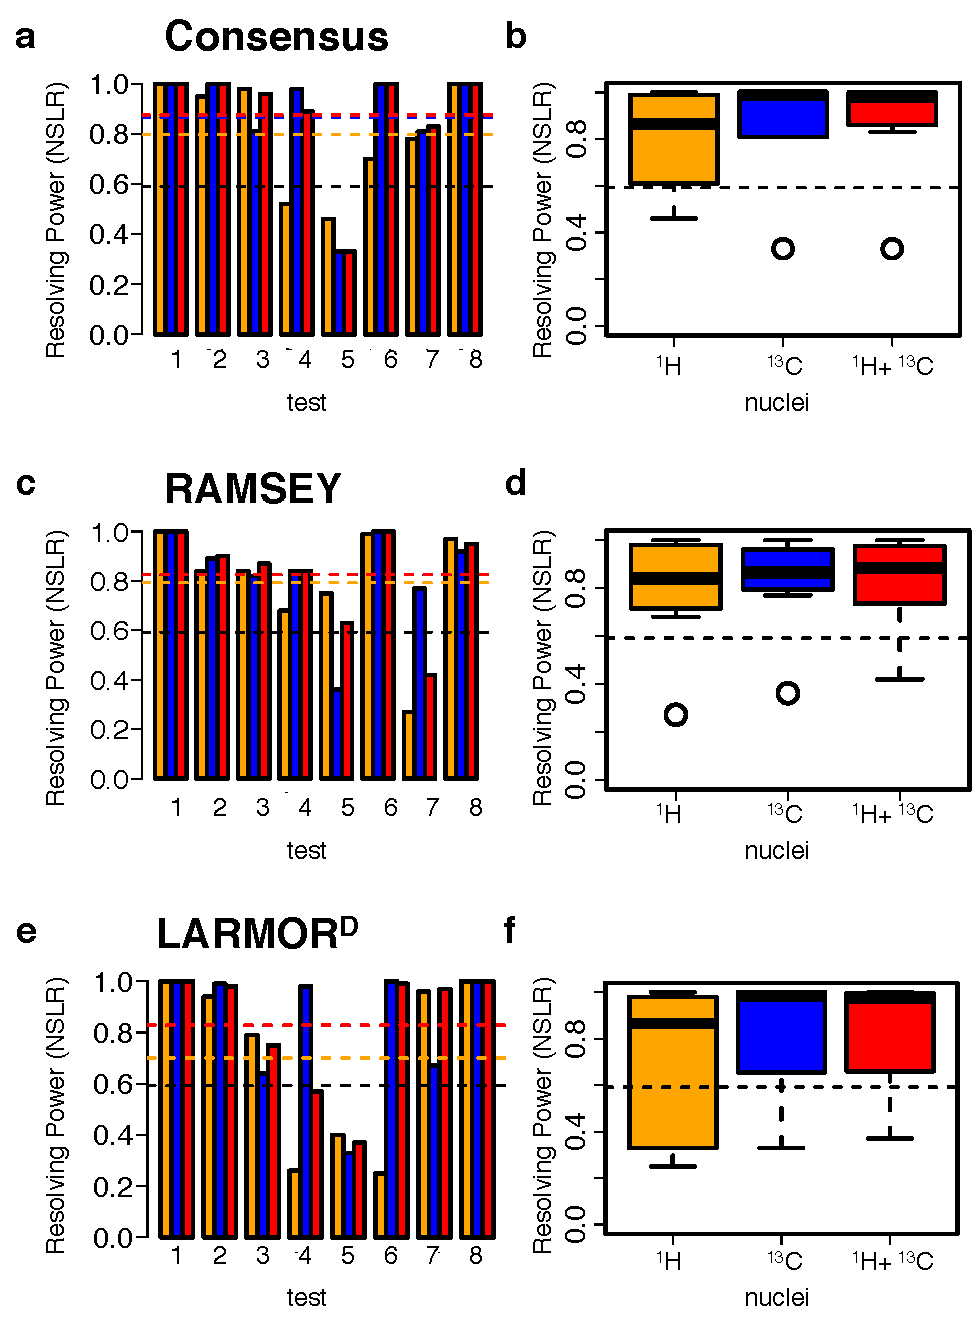
\includegraphics[width=0.5\textwidth]{figure_supplement_nslr}
\end{center}
\caption{ Results obtained when using reduced chemical shift errors between the observed and the (a and b) Consensus, (c and d) RAMSEY, and (e and f) LARMOR$^{\rm D}$ computed chemical shifts, to partition and ``resolve'' the pairs of related NMR structures in each of the eight test cases. In each pair of every test, the ``reference'' NMR structure is known to be more accurate (or consistent) with the observed (``reference") chemical shifts used to determine the chemical shift errors. Resolving scores close to 1 occur when most of models in the ``reference'' NMR structure have lower chemical shift error values than the other (comparison) NMR structure. Barplots of the ``resolving scores'' for the eight independent test cases examined in this study. Boxplot showing the distribution of scores shown in the barplot. Results are shown for scores computed based on $^{1}$H (orange), $^{13}$C (blue), and both$^{1}$H and $^{13}$C (red) the chemical shift errors.}
\label{fig:supporting_nslr}
\end{figure}
\clearpage

\begin{figure}[h]
\begin{center}
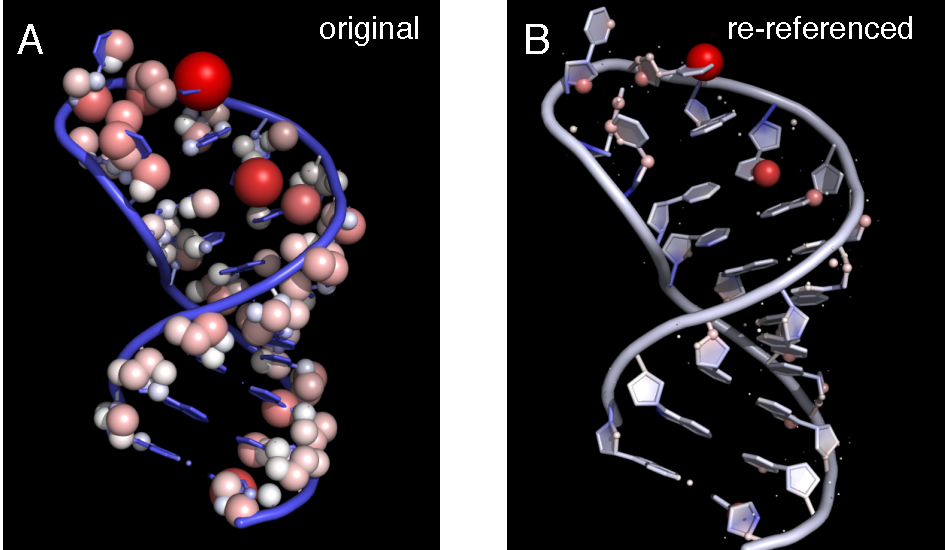
\includegraphics[width=0.5\textwidth]{figure_supplement_referencing}
\end{center}
\caption{ Visualizing referencing errors using PyShifts. Figure illustrating how referencing errors in chemical shift data can be visualized by computing chemical shift errors and then projecting them onto structural models. Cartoon representation of a test RNA with known $^{13}$C referencing errors (A) before and (B) after re-referencing the chemical shift data. Figures were generated using our Pymol plugin, PyShifts.}
\label{fig:supporting_nslr}
\end{figure}
\clearpage

\end{document}